\chapter{Etapas del proyecto: división en sprints y seguimiento de los mismos}\label{chapter:sprints}
\addcontentsline{toc}{chapter}{Etapas del proyecto: división en sprints}

El proyecto se ha dividido en once sprints de tres semanas cada uno y un último sprint con los días restantes. Además, durante el transcurso de cada sprint se ha realizado un seguimiento del trabajo realizado en el mismo, aportando \emph{burndown charts} de cada uno de ellos.

Un \emph{burdown chart} es una gráfica en la que se muestra el progreso de un proyecto durante cierto periodo de tiempo preestablecido (un sprint, una release o el proyecto completo, por ejemplo). Para la construcción de los mismos se requieren los siguientes elementos:
\begin{itemize}
\item El periodo de \emph{tiempo a analizar}, que se corresponderá con el eje X de la gráfica. El inicio del periodo temporal vendrá representado por $x = 0$ mientras que el final de dicho periodo será representado por $x = t$ donde $t$ es la duración del periodo. Si observamos el burndown chart global del proyecto (Figura global), estos dos valores se corresponderán, respectivamente, con las fechas de inicio y finalización del mismo.
\item La cantidad de trabajo a realizar, que se corresponderá con el eje Y de la gráfica y representa el trabajo planificado que se deberá realizar en el periodo de tiempo a analizar. Cuando se realiza la estimación de las tareas, independientemente de la unidad de estimación empleada, se obtiene una cantidad de trabajo a realizar (en horas, por ejemplo). Así pues, la cantidad de trabajo restante irá decreciendo conforme el tiempo vaya avanzando.
\item Una referencia ideal, que será la línea diagonal trazada desde la esquina superior izquierda hasta la esquina inferior derecha de la gráfica. Se trata de una representación de la relación ideal entre la disminución de la cantidad de trabajo y el tiempo dedicado durante el transcurso de la fase correspondiente. Esto es, cuanto más se aproxime la línea real a la ideal se estará trabajando de mejor manera en relación a la consecución de los objetivos marcados.
\end{itemize}

Adicionalmente, si se poseen conocimientos y experiencia trabajando con herramientas ágiles, se puede obtener información útil en ellas sobre el seguimiento del proyecto con el fin de impulsar buenas prácticas y mejorar el desarrollo del mismo.

\section{Análisis de cada sprint}

\begin{figure}[H]
\centering
\subfloat[Burndown chart del sprint 1 (periodo del 12/12/2022 al 01/01/2023).]{\label{fig:sprint1}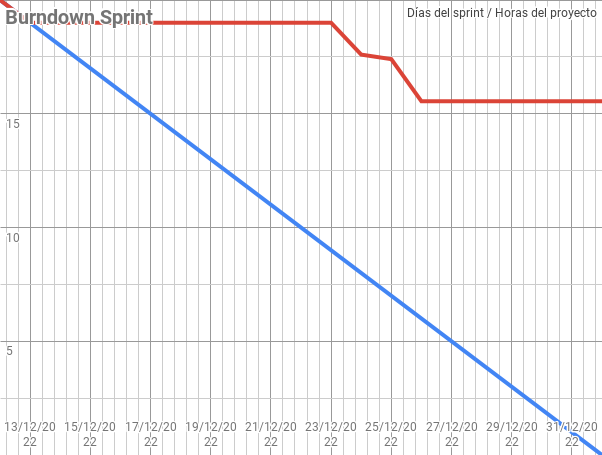
\includegraphics[width=0.46\textwidth]{sprints/Burndown Sprint 1.png}}\qquad
\subfloat[Burndown chart del sprint 2 (periodo del 02/01/2023 al 22/01/2023).]{\label{fig:sprint2}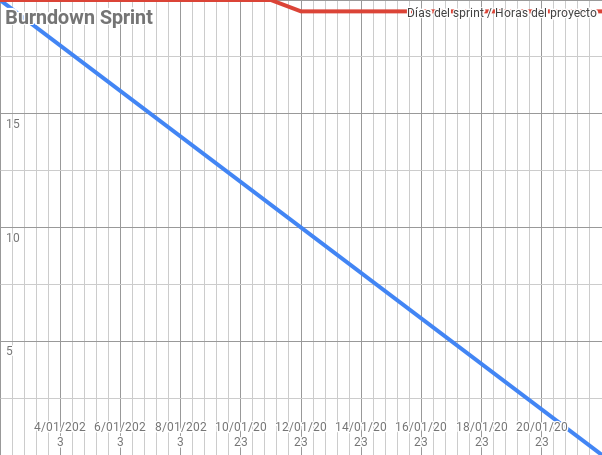
\includegraphics[width=0.46\textwidth]{sprints/Burndown Sprint 2.png}}\qquad
\subfloat[Burndown chart del sprint 3 (periodo del 23/01/2023 al 12/02/2023).]{\label{fig:sprint3}
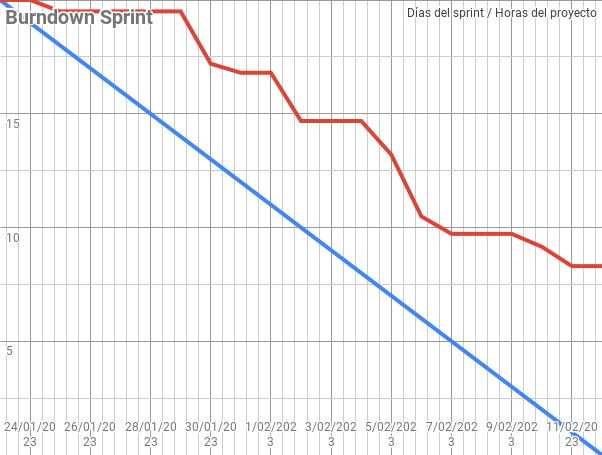
\includegraphics[width=0.46\textwidth]{sprints/Burndown Sprint 3.png}}\qquad
\subfloat[Burndown chart del sprint 4 (periodo del 13/02/2023 al 05/03/2023).]{\label{fig:sprint4}
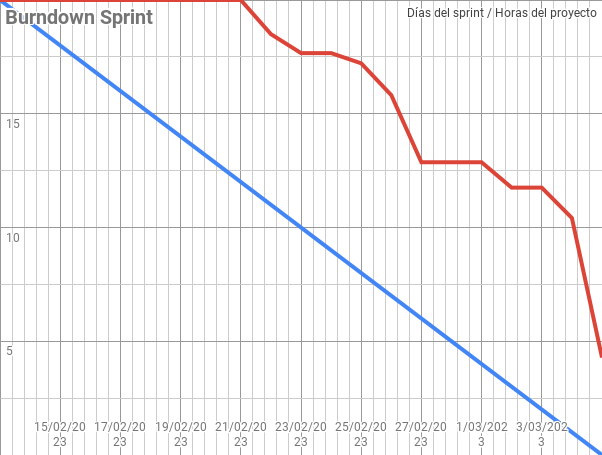
\includegraphics[width=0.46\textwidth]{sprints/Burndown Sprint 4.png}}\qquad
\subfloat[Burndown chart del sprint 5 (periodo del 06/03/2023 al 26/03/2023).]{\label{fig:sprint5}
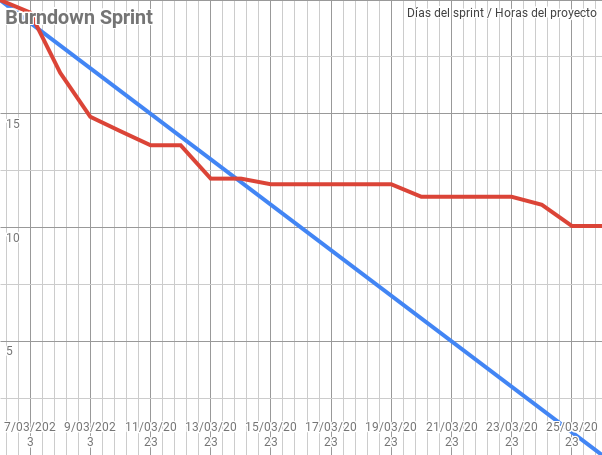
\includegraphics[width=0.46\textwidth]{sprints/Burndown Sprint 5.png}}\qquad
\subfloat[Burndown chart del sprint 6 (periodo del 27/03/2023 al 16/04/2023).]{\label{fig:sprint6}
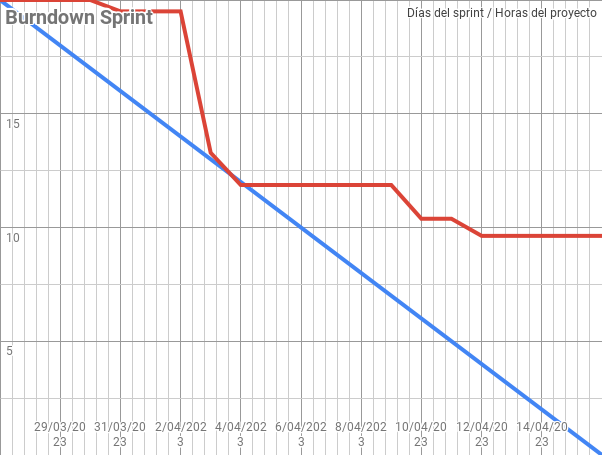
\includegraphics[width=0.46\textwidth]{sprints/Burndown Sprint 6.png}}
\caption{Burdown charts de los seis primeros sprints del proyecto.}
\label{fig:sprints1-6}
\end{figure}

\subsection{Sprint 1 (Figura \ref{fig:sprint1})}

Este primer sprint representa una situación anómala que no se debería dar. La explicación es sencilla: las líneas rojas horizontales representan periodos de tiempo en los cuales no se ha estado trabajando en el proyecto. No obstante, esto es correcto puesto que aunque se definieron unos objetivos al principio, todavía no tenía claro el procedimiento a seguir para la consecución de los mismos. Aunque podría haberse omitido este periodo de seguimiento, se ha decidio incluirlo como muestra de una tendencia no deseable en relación al desarrollo de un proyecto.

\subsection{Sprint 2 (Figura \ref{fig:sprint2})}

En este segundo sprint tampoco se han alcanzado los objetivos de trabajo preestablecidos. No obstante, es correcto porque este periodo coincide con la realización de exámenes y se planificó previamente para el estudio de los mismos y no para continuar con la realización de este trabajo fin de grado. Como se ha comentado anteriormente, durante el desarrollo de un proyecto, esta situación no debería ocurrir bajo ninguna circunstancia.

\subsection{Sprint 3 (Figura \ref{fig:sprint3})}

En este caso, la Figura \ref{fig:sprint3} muestra que se realizó una gran cantidad de trabajo focalizada en días concretos distribuidos a lo largo de todo el sprint con algunos parones entre medias. Sin embargo, a pesar de todo, no se consiguió llegar a la cantidad estipulada de trabajo al final del sprint.

\subsection{Sprint 4 (Figura \ref{fig:sprint4})}

Este cuarto sprint consiste en un periodo inicial inactivo seguido de varios picos de productividad en días concretos del sprint. Finalmente, podemos observar que se realizó una gran cantidad de trabajo al final del sprint, quedándose muy cerca la cantidad de trabajo realizada de la referencia ideal.

\subsection{Sprint 5 (Figura \ref{fig:sprint5})}

En este sprint podemos ver que se realizó más trabajo del requerido durante el primer tercio del mismo. Sin embargo, a partir de entonces, a pesar de que se avanza en días concretos, el ritmo de trabajo es mucho más lento y se termina por no realizar la cantidad de trabajo planificado durante dicho periodo temporal.

\subsection{Sprint 6 (Figura \ref{fig:sprint6})}

La gráfica de este sprint (Figura \ref{fig:sprint6}) muestra que se realizó una gran cantidad de trabajo al principio del sprint llegando la curva de trabajo real a cortar a la curva ideal un poco antes de la mitad de la misma. No obstante, al final del sprint hubo algún día de parón y el ritmo de trabajo se redujo. En consecuencia, no se alcanzaron los objetivos preestablecidos.

\begin{figure}[H]
\centering
\subfloat[Burndown chart del sprint 7 (periodo del 17/04/2023 al 07/05/2023).]{\label{fig:sprint7}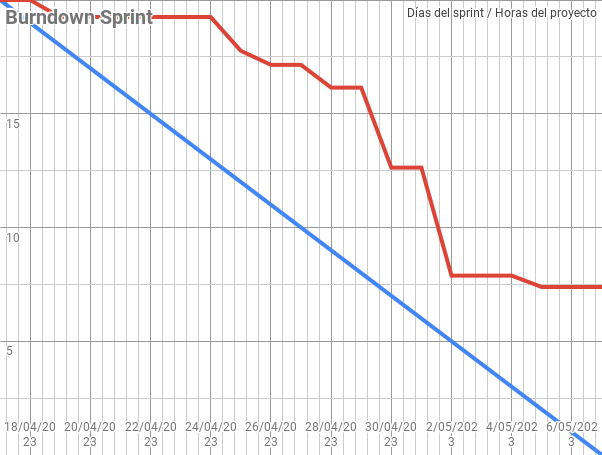
\includegraphics[width=0.46\textwidth]{sprints/Burndown Sprint 7.png}}\qquad
\subfloat[Burndown chart del sprint 8 (periodo del 08/05/2023 al 28/05/2023).]{\label{fig:sprint8}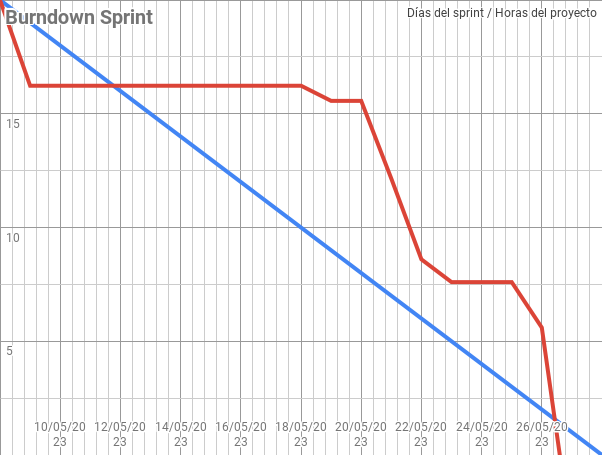
\includegraphics[width=0.46\textwidth]{sprints/Burndown Sprint 8.png}}\qquad
\subfloat[Burndown chart del sprint 9 (periodo del 29/05/2023 al 18/06/2023).]{\label{fig:sprint9}
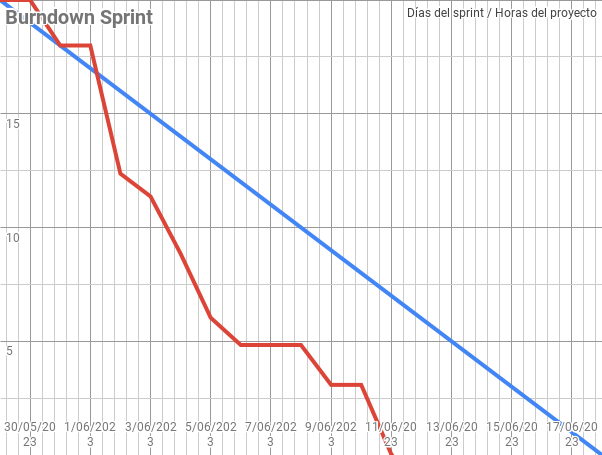
\includegraphics[width=0.46\textwidth]{sprints/Burndown Sprint 9.png}}\qquad
\subfloat[Burndown chart del sprint 10 (periodo del 19/06/2023 al 09/07/2023).]{\label{fig:sprint10}
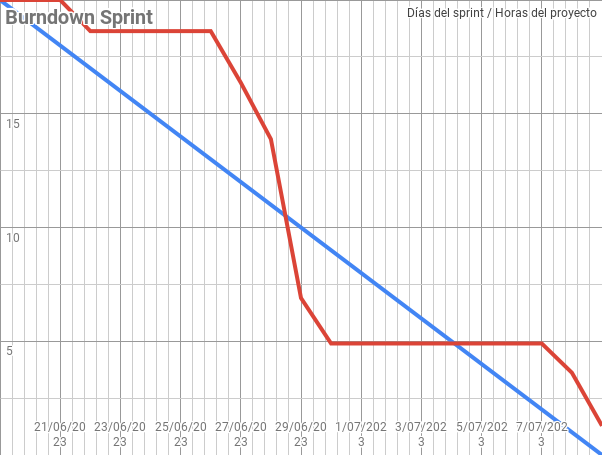
\includegraphics[width=0.46\textwidth]{sprints/Burndown Sprint 10.png}}\qquad
\subfloat[Burndown chart del sprint 11 (periodo del 10/07/2023 al 30/07/2023).]{\label{fig:sprint11}
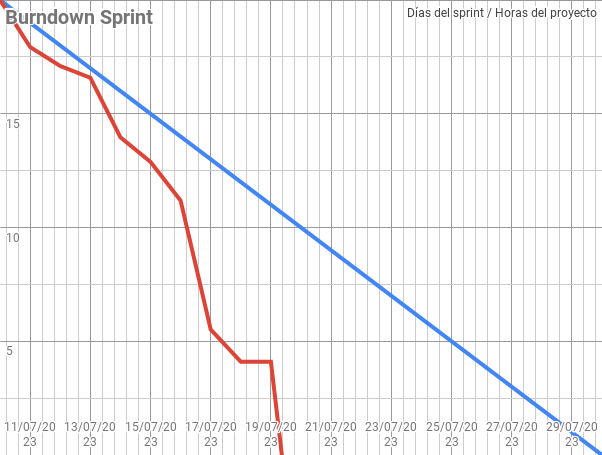
\includegraphics[width=0.46\textwidth]{sprints/Burndown Sprint 11.png}}\qquad
\subfloat[Burndown chart del sprint 12 (periodo del 31/07/2023 al 10/08/2023).]{\label{fig:sprint12}
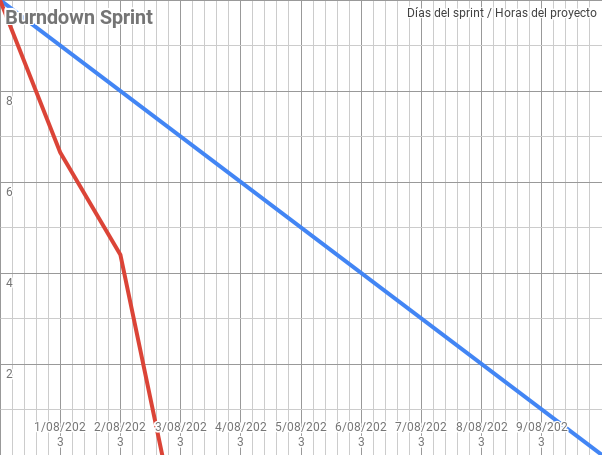
\includegraphics[width=0.46\textwidth]{sprints/Burndown Sprint 12.png}}
\caption{Burdown charts de los seis últimos sprints del proyecto.}
\label{fig:sprints7-12}
\end{figure}

\subsection{Sprint 7 (Figura \ref{fig:sprint7})}

En este caso, la Figura \ref{fig:sprint7} revela que hubo un ritmo de trabajo insuficiente tanto al principio como al final del sprint. Sin embargo, durante todo el tramo central del mismo se estuvo trabajando de manera intensa aunque insuficiente para abarcar toda la cantidad de trabajo asignada a este sprint.

\subsection{Sprint 8 (Figura \ref{fig:sprint8})}

En este octavo sprint podemos apreciar que se realiza más trabajo del planificado en los extremos del periodo considerado gracias a la realización de grandes esfuerzos en días concretos. Esto, en cierto modo, ha servido para compensar parte del trabajo no realizado durante la parte central del sprint.

\subsection{Sprint 9 (Figura \ref{fig:sprint9})}

Podemos ver claramente en la Figura \ref{fig:sprint9} que durante el periodo de tiempo asignado a este sprint se ha realizado mucho más trabajo del planificado. No obstante, realizando un análisis global del proyecto, este exceso de trabajo puede verse como una compensación del trabajo no completado en sprints anteriores.

\subsection{Sprint 10 (Figura \ref{fig:sprint10})}

Durante el décimo sprint se mantuvo una tendencia algo sosegada durante el primer cuarto del mismo. Sin embargo, después se aceleró el ritmo de tal forma que se cortaron la curva de trabajo real y la curva ideal hacia la mitad del sprint. Por último, tras relajarse el ritmo de trabajo se produce una recuperación del mismo, llegando a ser casi ideal hacia el final del sprint.

\subsection{Sprint 11 (Figura \ref{fig:sprint11})}

Al igual que en el noveno sprint, podemos observar que se realiza bastante más trabajo del asignado. Efectivamente, comparando las Figuras \ref{fig:sprint9} y \ref{fig:sprint11} podemos ver que la tendencia es parecida. Esto se debe a que, en las últimas fases del proyecto, se han dedicado una mayor cantidad de horas de trabajo con la finalidad de completarlo.

\subsection{Sprint 12 (Figura \ref{fig:sprint12})}

Este sprint tiene una duración menor a las tres semanas habituales de los sprints anteriores. Su longitud menor se debe a que se trata del último sprint del proyecto o sprint de finalización. Del mismo modo que ocurría en el sprint anterior, la cantidad de horas invertidas en el proyecto supera a la cantidad de horas que se planificaron inicialmente. No obstante, si se analiza desde un punto de vista global, el exceso de horas invertidas en los últimos sprints del proyecto compensa la cantidad de trabajo que no se llegó a completar en sprints anteriores.

\section{Análisis global del proyecto}

Observando el burndown chart global del proyecto (Figura \ref{fig:global}) se puede apreciar que hay algunos tramos de la curva completamente planos correspondientes a periodos de inactividad tal y como se ha mencionado anteriormente. Como consecuencia, puede apreciarse que hasta prácticamente el final del mismo se ha ido por detrás del trabajo planificado. No obstante, al final de su desarrollo se ha realizado más trabajo del estimado, aproximándose cada vez la curva de trabajo real a la curva ideal compensando finalmente la diferencia entre ambas.

Así pues, se puede concluir que globalmente se ha realizado la cantidad de trabajo estimada antes de la finalización del proyecto. Adicionalmente, pese al distanciamiento de la situación ideal en algunos puntos del mismo, se ha logrado mantener bajo control el proyecto durante los diferentes sprints. Finalmente, gracias al seguimiento realizado se han podido valorar en cada punto de su desarrollo los riesgos existentes, tomándose así medidas en relación a éstos, por ejemplo, compensando con trabajo extra las horas no empleadas en periodos anteriores.

\begin{figure}[H]
    \centering
    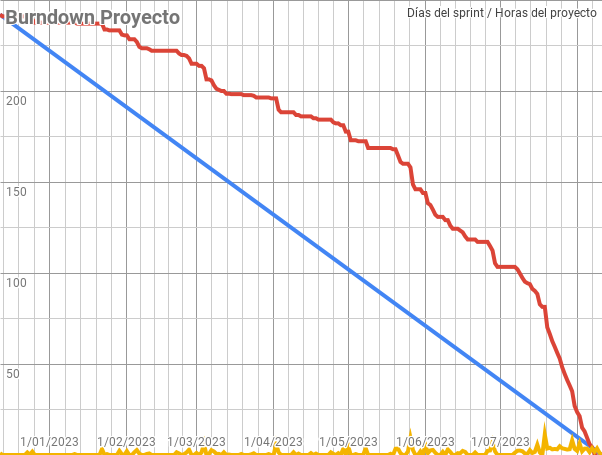
\includegraphics[width=0.60\textwidth]{sprints/Burndown Proyecto.png}
    \caption{Burndown chart del proyecto (periodo del 12/12/2022 al 10/08/2023).}
    \label{fig:global}
\end{figure}